\documentclass[11pt]{article}
\usepackage{amsmath, amssymb, array}
\pagestyle{plain}

\textwidth=6.5in
\hoffset-1in
\textheight=9in
\voffset-1in

\usepackage{enumitem}
\usepackage{pgfplots}
\usepackage{graphicx}
\usepackage{lipsum}
\usepackage{stfloats}
\usepackage{multicol}
\usepackage{minipage-marginpar}
\usepackage{tikz}
\setlength{\columnsep}{1cm}
\usepackage{pinlabel} % for pin labels on figure


\newcommand{\abs}[1]{\left| #1 \right|}


\begin{document}


\noindent MATH 1113   \quad\quad\quad\quad\quad Worksheet \quad\quad\quad\quad\quad\   Name \underline{\phantom{alphabetsoupismyveryveryfavorite}}\\ 
\noindent Section 2.3 \\




\noindent \textbf{Instructions:}  Work together in groups of  3 or 4 to complete the following problems.\\

\begin{enumerate}



\item Divide using long division.
\begin{enumerate}
\item $(8x^3-16x^2+2x-30)\div (2x-5)$
\vfill

\item $\displaystyle \frac{2x^4-3x^2+3x}{x-2}$
\vfill

\end{enumerate}

\newpage


\item Divide using synthetic division.

\begin{enumerate}

\item $(x^3+9x^2-7x+7)\div (x-6)$
\vfill
\item $\displaystyle \frac{x^5+7x^3-8}{x+1}$
\vfill

\end{enumerate}

\item Use synthetic division and the Remainder Theorem to find the indicated function value.
\begin{enumerate}
\item $f(x)=5x^3-13x^2+5x-6$; $f(1)$
\vfill
\item $f(x)=5x^4-29x^3-x^2+6x+4$; $\displaystyle f(-\frac{1}{5})$
\end{enumerate}

\vfill

\newpage
\item Solve the equation $x^3-5x^2+2x+8=0$ given that -1 is a zero of $f(x)=x^3-5x^2+2x+8$.

\vfill


\item Use the graph of $y=x^3+6x^2-7x-60$ to determine a solution of
  the equation
  $$x^3+6x^2-7x-60=0.$$
  Use synthetic division to verify that this number is a solution of
  the equation.

    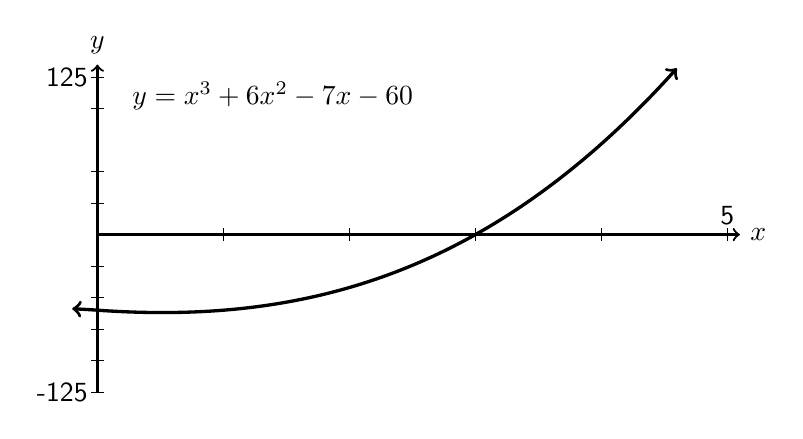
\begin{tikzpicture}[y=0.08cm, x=0.08cm,font=\sffamily]

    \begin{scope}[shift={(0,0)},xscale=20,yscale=0.2]
      %\draw[xstep = 2,ystep=5, gray, very thin,opacity=0.85] (0,40) grid (16,90);
      \draw[thick,black,->] (0,0) -- (5.1,0) node[anchor=west] {$x$};
      \draw[thick,black,->] (0,-125) -- (0,135) node[anchor=south] {$y$};

      %% Label the y axis
      \foreach \y in {-125,-100,-75,-50,-25,25,50,100,125} {
        \draw (0.05, \y) -- (-0.05, \y);
      }
      %% Label the x axis
      \foreach \x in {1,2,3,4,5} {
        \draw (\x,-5) -- (\x,5);
      }

      \node[black,anchor=south] at (5,0) {5};
      \node[black,anchor=east] at (0,-125) {-125};
      \node[black,anchor=east] at (0,125) {125};
      \node[black,anchor=west] at (0.2,110) {$y=x^3+6x^2-7x-60$};
    \end{scope}

    \begin{scope}[shift={(0,0)},xscale=20,yscale=0.2]
      \draw[scale=1.0,domain=-0.2:4.6,smooth,variable=\x,very thick,black,samples=120,<->] 
            plot ({\x},{\x^3+6*\x^2-7*\x-60});
    \end{scope}


  \end{tikzpicture}

\vfill

\newpage

\item Use the table below to determine a solution of the equation
  $$48x^3-110x^2+29x-2=0.$$
  Use synthetic division to verify that this number is a solution of
  the equation.

  \begin{tabular}[h]{r|rr}
    x & \multicolumn{2}{l}{$y=48x^3-110x^2+29x-2$} \\ \hline
    -3 & -2375 \\
    -2 & -884  \\
    -1 & -189 \\
     0 & -2 \\
     1 & -35 \\
     2 & 0 \\
     3 & 391
  \end{tabular}
\vfill

\item Use the factor theorem to determine if the given binomial is a factor of the polynomial $f(x)=x^4+11x^3+41x^2+61x+30$.
\begin{enumerate}
\item $x+5$
\vfill
\item $x-2$
\vfill

\end{enumerate}

\newpage

\item Consider the polynomial $f(x) = x^5 - 4x^4 - 3x^3+18x^2$.

\begin{enumerate}
	\item Describe the end behavior of the graph of $f(x)$.
	\vfill
	\item Use the Factor Theorem to determine if $x-3$ is a factor of $f(x)$
	\vfill
	\item Use long or synthetic division to factor $f(x)$.  (Hint: You need to know a factor.)
	\vfill
	\item Find all of the zeros for $f(x)$ and determine their multiplicity.
	\vfill
	\item Sketch a graph of $f(x)$. (Axes are given on the back.)
\end{enumerate}





\newpage

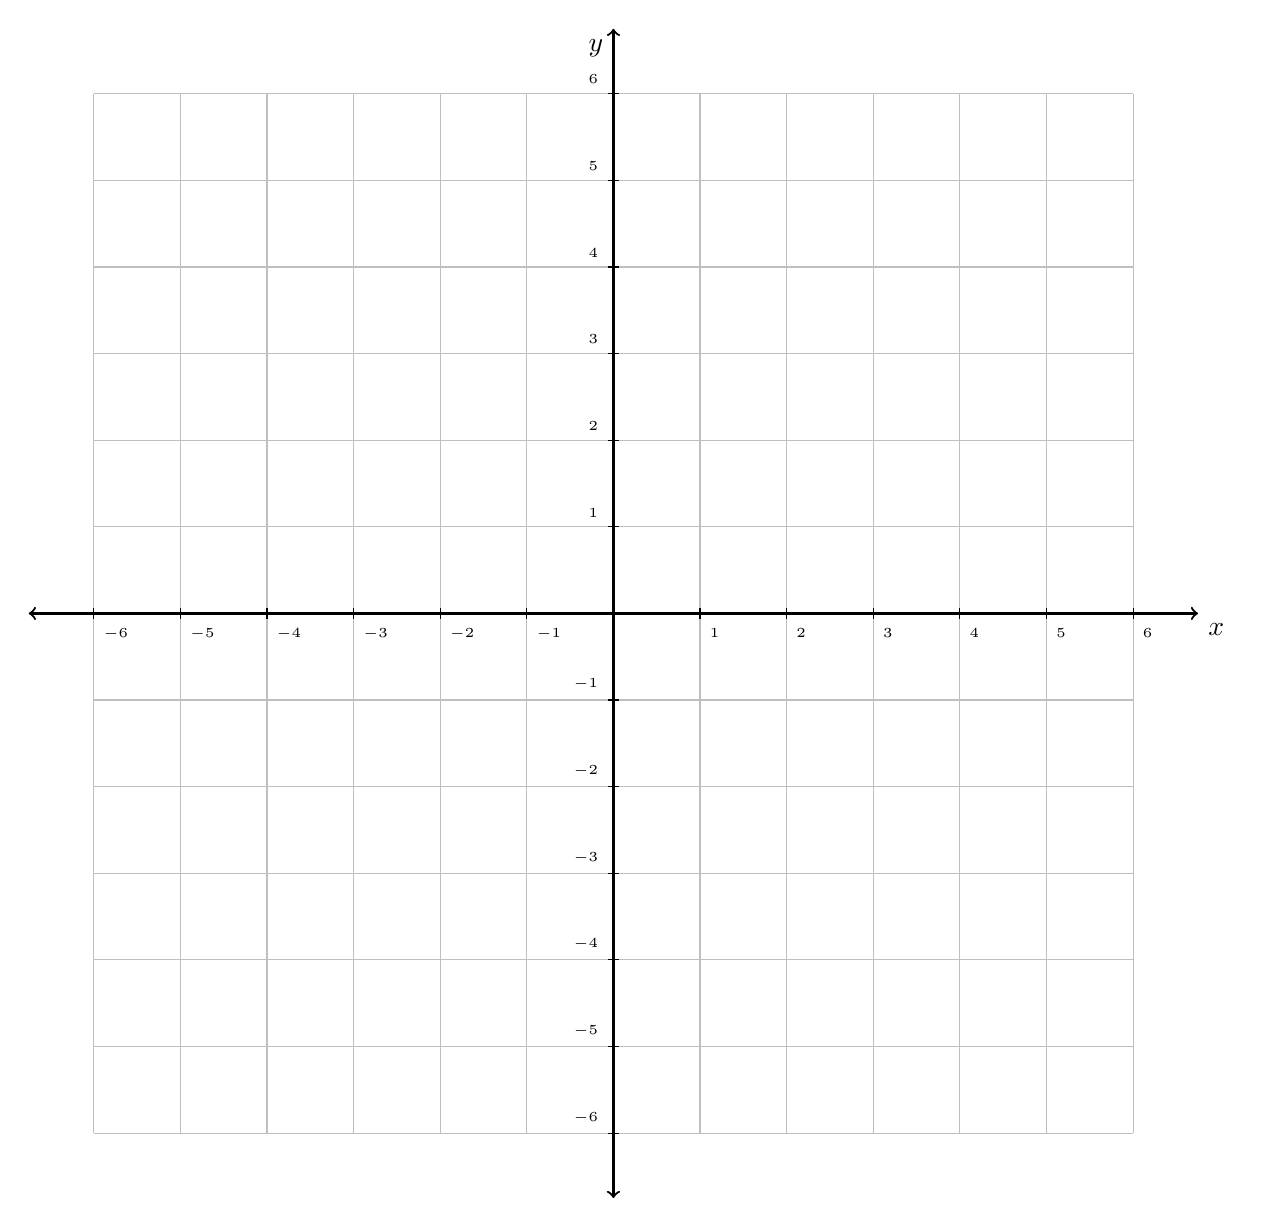
\begin{tikzpicture}[y=1.1cm, x=1.1cm,font=\sffamily]
    %% ticks
    \draw[step = 1, lightgray] (-6,-6) grid (6,6);
    %% axis
    \draw[thick,<->] (-6.75,0) -- coordinate (x axis mid) (6.75,0) node[anchor = north west] {$x$};
    \draw[thick,<->] (0,-6.75) -- coordinate (y axis mid) (0,6.75) node[anchor = north east] {$y$};
    \foreach \y in {-6,...,-1,1,2,...,6} {
      \draw (2pt, \y) -- (-2pt, \y) node[anchor =  south east] {\tiny$\y$};
    }
    \foreach \x in {-6,...,-1,1,2,...,6} {
      \draw (\x,2pt) -- (\x,-2pt) node[anchor =  north west] {\tiny$\x$};
    }

  \end{tikzpicture}
%\newpage
%
%\item Write a polynomial $f(x)$ that meets the given conditions.  (There are multiple correct answers.)
%\begin{enumerate}
%\item Degree 3 polynomial with zeros 2, 3, and -4
%\vfill
%\item Degree 4 polynomial with zeros 1, $\frac{3}{2}$ (each with multiplicity 1), and 0 (with multiplicity 2)
%\vfill
%
%\end{enumerate}
%
%
%
%\item Find $m$ so that $x+4$ is a factor of $4x^3+13x^2-5x+m$.
%\vfill
%\vfill
%\vfill

\newpage

%\item
%\begin{enumerate}
%\item Factor $f(x)=x^3-5x^2+x-5$ into factors of the form $(x-c)$, given that 5 is a zero.
%\vfill
%\item  Solve $x^3-5x^2+x-5=0$
%\vfill
%\end{enumerate}
%
%
%\item
%\begin{enumerate}
%\item Factor $f(x)=x^4+2x^3-2x^2-6x-3$ into factors of the form $(x-c)$, given that -1 is a zero.
%\vfill
%\item  Solve $x^4+2x^3-2x^2-6x-3=0$
%\vfill
%\end{enumerate}




\end{enumerate}

\end{document}
